\documentclass[12pt,a4paper]{amsart}
% ukazi za delo s slovenscino -- izberi kodiranje, ki ti ustreza
\usepackage[slovene]{babel}
%\usepackage[cp1250]{inputenc}
\usepackage[T1]{fontenc}
\usepackage[utf8]{inputenc}
\usepackage{amsmath,amssymb,amsfonts}
\usepackage{url}
%\usepackage[normalem]{ulem}
\usepackage[dvipsnames,usenames]{color}
\usepackage{graphicx}

% ne spreminjaj podatkov, ki vplivajo na obliko strani
\textwidth 15cm
\textheight 24cm
\oddsidemargin.5cm
\evensidemargin.5cm
\topmargin-5mm
\addtolength{\footskip}{10pt}
\pagestyle{plain}
\overfullrule=15pt % oznaci predlogo vrstico


% ukazi za matematicna okolja
\theoremstyle{definition} % tekst napisan pokoncno
\newtheorem{definicija}{Definicija}[section]
\newtheorem{primer}[definicija]{Primer}
\newtheorem{opomba}[definicija]{Opomba}

\theoremstyle{plain} % tekst napisan posevno
\newtheorem{lema}[definicija]{Lema}
\newtheorem{izrek}[definicija]{Izrek}
\newtheorem{trditev}[definicija]{Trditev}
\newtheorem{posledica}[definicija]{Posledica}


% za stevilske mnozice uporabi naslednje simbole
\newcommand{\R}{\mathbb R}
\newcommand{\N}{\mathbb N}
\newcommand{\Z}{\mathbb Z}
\newcommand{\C}{\mathbb C}
\newcommand{\Q}{\mathbb Q}


% naslednje ukaze ustrezno popravi
\newcommand{\program}{Matematika} % ime studijskega programa: Matematika/Finan"cna matematika
\newcommand{\imeavtorja}{Ines Meršak} % ime avtorja
\newcommand{\imementorja}{prof.~dr. Sandi Klavžar} % akademski naziv in ime mentorja
\newcommand{\naslovdela}{Problem londonskega stolpa}
\newcommand{\letnica}{2016} %letnica diplome


% commands
\newcommand{\graf}[1][G]{\ensuremath{#1 = (V(#1), E(#1))}}
\newcommand{\vozlisca}[1][G]{\ensuremath{V(#1)}}
\newcommand{\povezave}[1][G]{\ensuremath{E(#1)}}
\newcommand{\bd}{\ensuremath{|\,}}
\newcommand{\ed}{\ensuremath{\,|}}
% operatorji
\DeclareMathOperator {\stopnja} {deg}




\begin{document}

% od tod do povzetka ne spreminjaj nicesar
\thispagestyle{empty}
\noindent{\large
UNIVERZA V LJUBLJANI\\[1mm]
FAKULTETA ZA MATEMATIKO IN FIZIKO\\[5mm]
\program\ -- 1.~stopnja}
\vfill

\begin{center}{\large
\imeavtorja\\[2mm]
{\bf \naslovdela}\\[10mm]
Delo diplomskega seminarja\\[1cm]
Mentor: \imementorja}
\end{center}
\vfill

\noindent{\large
Ljubljana, \letnica}
\pagebreak

\thispagestyle{empty}
\tableofcontents
\pagebreak

\thispagestyle{empty}
\begin{center}
{\bf \naslovdela}\\[3mm]
{\sc Povzetek}
\end{center}
% tekst povzetka v slovenscini
V povzetku na kratko opi"si vsebinske rezultate dela. Sem ne sodi razlaga organizacije dela -- v katerem poglavju/razdelku je kaj, pa"c pa le opis vsebine.
\vfill
\begin{center}
{\bf The Tower of London problem}\\[3mm] % prevod slovenskega naslova dela 
{\sc Abstract}
\end{center}
% tekst povzetka v anglescini
Prevod zgornjega povzetka v angle"s"cino.

\vfill\noindent
{\bf Math. Subj. Class. (2010):} navedi vsaj eno klasifikacijsko oznako -- dostopne so na \url{www.ams.org/mathscinet/msc/msc2010.html}  \\[1mm]  
{\bf Klju"cne besede:} navedi nekaj klju"cnih pojmov, ki nastopajo v delu  \\[1mm]  
{\bf Keywords:} angle"ski prevod klju"cnih besed
\pagebreak


 
% tu se zacne tekst seminarja
\section{Uvod}
Test londonskega stolpa je ena izmed variacij Hanojskih stolpov. Izumil ga je britanski nevropsiholog Tim Shallice leta 1982. Pogosto je uporabljen v psihologiji, saj s pomočjo te igre ugotavljajo stanje pacientove psihe, opazujejo pa lahko tudi napredek bolezni pri npr.\ Parkinsonovih bolnikih. \cite{bib:wikishal}

Osnovna verzija londonskega stolpa vsebuje tri enako velike krogle različnih barv in tri palice. Na prvo palico lahko postavimo samo eno kroglo, na drugo le dve krogli, na tretjo pa tri. Cilj igre je priti iz nekega danega stanja v neko drugo želeno stanje s čim manj koraki. Stanja (in prehode med njimi) lahko opišemo s pomočjo teorije grafov.

Diplomska naloga je razdeljena na tri dele: v prvem delu bom najprej opisala vse pojme, navedla (in nekatere tudi dokazale) vse trditve, izreke in posledice teorije grafov, ki mi bodo v pomoč pri obravnavi problema londoskega stolpa. V drugem delu bom podrobneje opisala klasični londonski stolp in lastnosti pripadajočega grafa, v zadnjem delu pa bom obravnavala posplošeni problem londonskega stolpa.


\section{Osnovni pojmi teorije grafov}

Vsa možna stanja londonskega stolpa in prehode med njimi lahko zelo elegantno opišemo s pomočjo grafov, zato si najprej poglejmo nekaj osnovnih pojmov teorije grafov.

\begin{definicija}
	\emph{Graf} $G$ je urejen par $(\vozlisca, \povezave)$, kjer je $\vozlisca$ končna množica \emph{vozlišč}, $\povezave$ pa množica \emph{povezav} grafa. Povezave so predstavljene kot neurejeni pari vozlišč (neusmerjeni grafi).
\end{definicija}

Obstajajo variacije zgornje definicije, graf je lahko npr.\ usmerjen (povezave so urejeni pari) -- tedaj govorimo o \emph{digrafih}, ima neskončno število vozlišč ali pa več povezav med dvema vozliščema. Dopuščamo lahko tudi zanke: to je povezava oblike $\{v,v\}$, pri čemer je $v$ vozlišče.

Vozlišča grafa predstavimo s točkami v ravnini, povezavo med dvema vozliščema pa kot enostavno krivuljo med ustreznima točkama v ravnini.

\begin{figure}[h]
    %\includegraphics[width=200pt]{img/basicgraph.png}
    \caption{Možna predstavitev grafa v ravnini.}
\end{figure}
    
Če je $e = \{ u,v \}$ povezava, tedaj sta $u$ in $v$ \emph{krajišči} povezave $e$, pišemo tudi $e = uv$; rečemo, da sta $u$ in $v$ \emph{sosednji vozlišči}.

\begin{definicija}
	\emph{Soseščina} vozlišča $u$ je množica vseh sosednjih vozlišč vozlišča $u$:
	\[ N(u) = \{ x\colon ux \in \povezave \} .\]
	\emph{Stopnja vozlišča} $u$ je število vseh vozlišč, ki so mu sosednji: $\stopnja u = |N(u)|$.
\end{definicija}

\begin{primer}
    \label{primer:sosedi}
    Naj bo graf $G$ podan z \[\vozlisca = \{ 1,2,3,4,5 \}, \quad \povezave = \left\{ \{1,4\},\{1,5\},\{2,5\},\{3,4\},\{3,5\} \right\}.\]
    \begin{figure}[h]
%        \includegraphics[width=200pt]{img/primer1.png}
        \caption{Graf $G$.}
    \end{figure}
    Soseščina vozlišča 5 je $N(5) = \{1,2,3\}$.
\end{primer}

\begin{definicija}
	Graf $\graf[H]$ je \emph{podgraf} grafa $\graf$, če velja 
	\[ \vozlisca[H] \subseteq \vozlisca \text{ in } \povezave[H] \subseteq \povezave. \]
	Podgraf H grafa G je \emph{inducirani} podgraf, če za vsaki dve vozlišči $x,y\in \vozlisca[H]$ velja: $xy \in \povezave \implies xy \in \povezave[H]$.
\end{definicija}

\begin{primer}
    Če vzamemo graf $G$ iz prejšnjega primera \ref{primer:sosedi}, potem je graf $H$, ki ima
    
    \[ \vozlisca[H] = \{2,3,4,5\},\quad \povezave[H] = \left\{ \{2,3\},\{2,5\},\{3,4\},\{3,5\} \right\} \]
    
    induciran podgraf grafa $G$.
    
    \begin{figure}[h]
        %     \includegraphics[width=200pt]{img/primer1.png}
%        \includegraphics[width=200pt]{img/primer2.png}
        \caption{Graf $H$ je induciran podgraf grafa $G$.}
    \end{figure}
\end{primer}

Poglejmo si nekaj razredov grafov, ki nam bodo prišli prav v kasnejših definicijah. 

\emph{Pot} na $n$ vozliščih je graf, ki ima dve vozlišči stopnje $1$, medtem ko so preostala vozlišča stopnje $2$.

\emph{Cikel} na $n$ vozliščih (označimo ga s $C_n$) je graf, ki ga dobimo iz poti na $n$ vozliščih tako, da dodamo povezavo med vozliščema stopnje $1$.

\emph{Polni graf} na $n$ vozliščih (označimo ga s $K_n$) je graf, za katerega velja 
\[ uv \in \povezave[K_n] \quad \forall u,v \in \vozlisca[K_n].\] 
Z besedami, vsa vozlišča polnega grafa so med sabo povezana.

\begin{figure}[h]
%    \includegraphics[width=200pt]{img/pot6.png}
%    \includegraphics[width=200pt]{img/cikel6.png}
    \caption{Primer poti (levo), cikla (sredina) in polnega grafa (desno) na šestih vozliščih.}
\end{figure}

\begin{definicija}
    Graf $G$ je \emph{dvodelen}, če lahko množico njegovih vozlišč razbijemo na dva dela ($V_1,V_2$) tako, da ima vsaka povezava grafa $G$ eno krajišče v $V_1$ in drugo v $V_2$.
\end{definicija}

Pri polnem dvodelnem grafu z $n$ vozlišči v prvi množici, recimo ji $V_1$, in $m$ vozlišči v drugi množici, recimo ji $V_2$, je vsako vozlišče iz množice $V_1$ povezano z vsakim iz $V_2$, medtem ko znotraj množic vozlišča niso povezana. Tak graf označimo s $K_{n,m}$.

\begin{figure}[h]
    %    \includegraphics[width=200pt]{img/polni-dvodelni-graf.png}
    \caption{Na sliki je polni dvodelni graf $K_{2,4}$.}
\end{figure}

\begin{definicija}
	Naj bosta $\graf$ in $\graf[H]$ grafa. 
	Preslikava $f\colon \vozlisca \to \vozlisca[H]$ je \emph{izomorfizem}, če je bijektivna in velja
	\[ uv \in \povezave \iff f(u)f(v) \in \povezave[H],\quad \forall u, v \in \povezave. \]
	Grafa $G$ in $H$ sta \emph{izomorfna}, če obstaja izomorfizem $G \to H$. Oznaka: $G \cong H$.
\end{definicija}

\emph{Pot v grafu} $G$ je podgraf grafa $G$, ki je izomorfen poti.
\emph{Cikel v grafu} $G$ je podgraf grafa $G$, ki je izomorfen ciklu. 

\subsection{Povezanost grafa}

\emph{Sprehod} v grafu $G$ je zaporedje vozlišč $v_1, v_2, \ldots, v_k$, tako da velja $v_i v_{i+1} \in E(G),$ pri čemer je $1 \leq i \leq k-1$. Če označimo $x = x_1$ in $y = x_k$, potem takemu sprehodu rečemo $x,y$-sprehod.

Sprehod je \emph{enostaven}, če so vsa njegova vozlišča različna. Enostaven sprehod inducira podgraf, ki je izomorfen poti (torej pot v grafu).

\begin{figure}[h]
%    \includegraphics[width=200pt]{img/enostaven-sprehod1.png}
%    \includegraphics[width=200pt]{img/enostaven-sprehod2.png}
    \caption{Enostaven sprehod in pot v grafu, ki jo inducira.}
\end{figure}

Naj bo $G$ graf in $\sim$ relacija, definirana na kartezičnem produktu $\vozlisca \times \vozlisca$:
\[ x \sim y \ \stackrel{\text{def}}{\equiv} \ \exists \ x,y \text{-sprehod.} \]

Preprosto lahko preverimo, da je relacija $\sim$ ekvivalenčna. Sledi, da relacija $\sim$ množico vozlišč grafa G razbije na ekvivalenčne razrede. Podgrafi, inducirani s temi razredi, so \emph{komponente} grafa $G$.

\begin{definicija}
	Graf je \emph{povezan}, če ima le eno komponento. Povedano drugače, za poljuben par vozlišč mora obstajati sprehod med njima.
\end{definicija}

\begin{figure}[h]
%    \includegraphics[width=200pt]{img/povezan-graf.png}
%    \includegraphics[width=200pt]{img/nepovezan-graf.png}
    \caption{Povezan (levo) in nepovezan (desno) graf.}
\end{figure}

Če je $G$ povezan graf, lahko definiramo \emph{razdaljo} $d_G(u,v)$ med vozliščema $u$ in $v$ kot najmanjše možno število povezav na neki $u,v$-poti.

\subsection{Hamiltonovi grafi}

Eno izmed zanimivih vprašanj v teoriji grafov je, ali je možno najti neko pot/cikel v grafu, ki vsebuje vsa vozlišča tega grafa. S tem problemom se je ukvarjal tudi Hamilton, po katerem so take poti in cikli poimenovani; njega je zanimalo predvsem, ali je mogoče poiskati cikel, ki vsebuje vsa vozlišča, v dodekaedru \cite{bib:wikihamilpath}.

\begin{definicija}
	Pot v grafu, ki vsebuje vsa vozlišča tega grafa, se imenuje \emph{Hamiltonova pot}.
	\emph{Hamiltonov cikel} nekega grafa $G$ je cikel v $G$, ki poteka skozi vsa vozlišča tega grafa.
	Graf je \emph{Hamiltonov}, če vsebuje Hamiltonov cikel.
\end{definicija}

Za Hamiltonove grafe velja naslednji izrek, ki je tudi potrebni pogoj za to, da graf vsebuje Hamiltonov cikel.

\begin{izrek}
	Naj bo $G$ Hamiltonov graf. Za vsako podmnožico vozlišč $X \subseteq V(G)$ velja, da ima graf $G \setminus X$ kvečjemu $|X|$ komponent.
\end{izrek}

\proof

\endproof

\subsection{Ravninski grafi}

V diplomski nalogi se bom ukvarjala tudi s tem, kdaj je graf, s pomočjo katerega predstavimo londonski stolp, ravninski.

\begin{definicija}
    Graf je \emph{ravninski}, če ga lahko narišemo v ravnini tako, da se nobeni povezavi ne križata.
\end{definicija}

Če je graf narisan v ravnini brez križanja povezav, rečemo, da je graf vložen v ravnino.

\begin{figure}[h]
%    \includegraphics[width=200pt]{img/k4.png}
    \caption{Ravninskost grafa $K_4$ ni očitna.}
\end{figure}

Hitro lahko vidimo, da grafa $K_5$ in $K_{3,3}$ nista ravninska (poskusimo ju narisati v ravnini, a kmalu ugotovimo, da to ne bo mogoče). To dejstvo sledi tudi kot posledica ene izmed posledic Eulerjeve formule.

Za začetek moramo najprej definirati \emph{lica vložitve}. To so sklenjena območja, ki jih omejuje risba grafa, vloženega v ravnino.

\begin{izrek}[Eulerjeva formula]
    Naj bo $G$ povezan ravninski graf z $n$ vozlišči in $m$ povezavami. Naj ima risba grafa $G$, vloženega v ravnino, $f$ lic. Potem velja
    \[ n - m + f = 2 .\]
\end{izrek}

Eulerjevo formulo dokažemo z indukcijo na število povezav, zaradi jedrnatosti besedila bomo dokaz tukaj izpustili. Oglejmo si raje posledico Eulerjeve formule:

\begin{posledica}
    Če je $G$ ravninski graf na $n$ vozliščih in $m$ povezavah, velja
    \[ m \leq 3n - 6 .\]
\end{posledica}

\begin{proof}
    Če za vsako lice upoštevamo le tri povezave (to je minimalno število povezav, ki omejujejo lice), bomo dobili kvečjemu manj, kot če preštejemo vse povezave dvakrat. Torej velja neenakost
    \[ 3f \leq 2m .\]
    Če iz Eulerjeve formule izrazimo $f$ in ga vstavimo v zgornjo neenakost, dobimo
    \begin{align*}
        3\cdot(2-n+m) &\leq 2m \\
        6 - 3n + 3m &\leq 2m \\
        m &\leq 3n - 6 \qedhere
    \end{align*}
\end{proof}

Z uporabo zgornje formule, ki torej mora veljati, če je graf ravninski, lahko dokažemo:
\begin{posledica}
    \label{posl:neravninska-grafa}
    $K_5$ in $K_{3,3}$ nista ravninska grafa.
\end{posledica}

Sedaj želimo ugotoviti, kakšnim pogojem mora ustrezati graf, da bo ravninski. Očitno velja naslednja trditev:

\begin{trditev}
    \label{trd:podgraf}
    Če je graf ravninski, potem je tudi vsak njegov podgraf ravninski. \cite{bib:potocnik}
\end{trditev}

Operacija ``podgraf'' torej ohranja ravninskost grafa.
Pogledali si bomo še operacijo \emph{subdivizije}, ki prav tako ohranja lastnost ravninskosti.

\begin{definicija}
    Graf $H$ je \emph{subdivizija} grafa $G$, če ga lahko dobimo iz $G$ tako, da povezave grafa $G$ nadomestimo s paroma notranje disjunktnimi potmi.
\end{definicija}

Iz definicije je razvidno, da je tak $H$ ravninski natanko tedaj, ko je $G$ ravninski. Iz tega dejstva, trditve \ref{trd:podgraf} in posledice \ref{posl:neravninska-grafa} lahko zaključimo, da graf zagotovo ni ravninski, če vsebuje subdivizijo $K_5$ ali $K_{3,3}$. Zanimivo pa je, da velja tudi obratno; dokaz tega dejstva je netrivialen in ga lahko najdemo v [TODO vir].

\begin{izrek}[Kuratowski]
    Graf G je ravninski natanko tedaj, ko ne vsebuje subdivizije $K_5$ niti subdivizije $K_{3,3}$.
\end{izrek}
%\begin{definicija}
%	\emph{Barvanje} grafa $\graf$ je preslikava 
%	\[ c\colon \vozlisca \to \N, \text{ tako da velja } av \in \povezave \implies c(a) \neq c(v). \]
%	Če je $c\colon \vozlisca \to [k]$, rečemo, da je $c$ $k$-barvanje. \emph{Kromatično število} grafa $G$, $\mathcal{X}(G)$, je najmanjši $k$, za katerega obstaja $k$-barvanje grafa G.
%\end{definicija}

\section{Klasični problem londonskega stolpa}
Pri klasičnem londonskem stolpu imamo tri enako velike krogle različnih barv in tri palice različnih velikosti: na prvo lahko postavimo eno kroglo, na drugo dve, na tretjo pa tri (temu bomo rekli, da imajo palice višine 1, 2 in 3). Cilj igre je priti iz nekega začetnega stanja v neko vnaprej določeno končno stanje.

\begin{figure}[h]
    
\includegraphics[width=250pt]{img/london-tower.png}
    \caption{Na sliki sta prikazani dve možni stanji londonskega stolpa.}
    \label{fig:stanji}
\end{figure}

Stanja in prehode med njimi si najlažje predstavljamo, če narišemo graf. V ta namen vpeljemo naslednje oznake:
krogle bomo označili s številkami 1, 2, 3 -- npr.\ modra krogla naj ima oznako 1, rdeča 2, rumena pa 3 -- s simbolom ``|'' pa bomo označili konec prejšnje palice in začetek nove. Krogle bomo naštevali od vrha palice navzdol.

\begin{primer}
    Začetno stanje na sliki \ref{fig:stanji} lahko torej opišemo z $\bd 3 \ed 12$, končno stanje pa z $\bd 21 \ed 3$.
\end{primer}

S pomočjo teh oznak lahko opišemo vsako možno stanje in narišemo graf londonskega stolpa (označimo ga z $L$), pri čemer so vozlišča stanja, povezave pa so med tistimi stanji, med katerimi lahko prehajamo z eno potezo (enim veljavnim premikom krogle).

\begin{figure}[h!]
    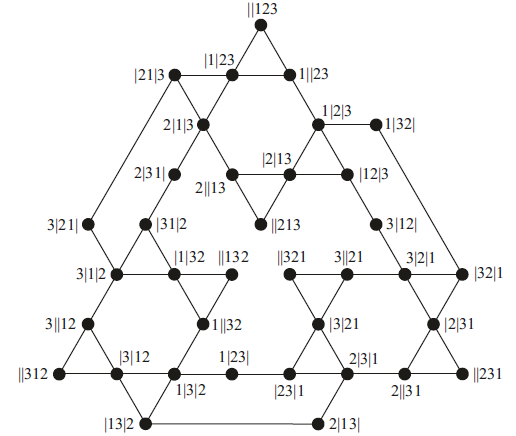
\includegraphics[width=300pt]{img/tolgraph.png}
    \caption{Graf $L$ klasičnega Londonskega stolpa.}
    \label{fig:tolgraph}
\end{figure}

Število vseh možnih stanj je 36, torej ima $L$ 36 vozlišč. Očitno je graf ravninski, saj je na sliki~\ref{fig:tolgraph} narisan v ravnini brez križanja povezav. Hitro vidimo tudi, da je 12 vozlišč grafa $L$ stopnje 2, drugih 12 je stopnje 3, zadnjih 12 pa stopnje 4.

\begin{primer}
    S pomočjo grafa na sliki \ref{fig:tolgraph} lahko hitro ugotovimo, da za prehod med stanjema na sliki \ref{fig:stanji} potrebujemo minimalno 4 poteze in da je to edino najkrajše možno zaporedje potez.
\end{primer}

\bigskip

\begin{trditev}
    Graf $L$ vsebuje Hamiltonovo pot, ne pa tudi Hamiltonovega cikla.
\end{trditev}

\section{Posplošeni londonski stolp}

\subsection{Definicija in osnovne lastnosti}

\begin{definicija}
    Za \emph{londonski graf} $L_h^n$, kjer je $p \geq 3,\ n \geq 2,\ h \in [n]^p,\  \sum_{k=1}^p h_k \geq n$ velja:
    \begin{itemize}
        \item vozlišča so vse permutacije $s \in S_{n+p}$, za katere velja:
        \[\forall k \in [p]:\ 1 \leq s_{n+k} - s_{n+k-1} \leq h_k + 1,\ s_{n+p} = n + p ,\]
        \item vsaki dve stanji (oz.\ pripadajoči permutaciji), med katerima lahko prehajamo z veljavno potezo, sta povezani
    \end{itemize}
\end{definicija}

Potreben pogoj za povezanost londonskega grafa je 
\[ n \leq \sum_{k=1}^{p-1} h_k. \]
\begin{izrek}
    Londonski graf $L_h^n$ je povezan natanko tedaj, ko velja pogoj
    \[ n \leq \sum_{k=1}^{p-1} h_k. \]
\end{izrek}

\subsection{Ravninskost londonskega grafa}

\begin{trditev}
    Naj bo $p=3$. Tedaj so londonski grafi $L_h^2, L_{122}^3,L_{123}^3$ in $ L_{133}^3$ ravninski.
\end{trditev}

\subsection{Simetrija londonskega stolpa}
% seznam uporabljene literature
\begin{thebibliography}{99}

\bibitem{bib:tohmyths} A. M. Hinz, S. Klavžar, U. Milutinović in C. Petr, \emph{The Tower of Hanoi – Myths and Maths}, Birkhäuser, Basel, 2013.

\bibitem{bib:potocnik} P. Potočnik, \emph{Zapiski predavanj iz Diskretne Matematike I}, 1.~izdaja, [ogled 29.~12.~15], dostopno na \url{http://www.fmf.uni-lj.si/~potocnik/Ucbeniki/DM-Zapiski2010.pdf}

\bibitem{bib:wikishal} \emph{Tim Shallice}, v: Wikipedia: The Free Encyclopedia, [ogled 8.~10.~2015], dostopno na\\ \url{https://en.wikipedia.org/wiki/Tim_Shallice}.

\bibitem{bib:wikihamilpath} \emph{Hamiltonian path}, v: Wikipedia: The Free Encyclopedia, [ogled 28.~12.~2015], dostopno na \url{https://en.wikipedia.org/wiki/Hamiltonian_path}.
\end{thebibliography}

\end{document}

